\documentclass{article}
\usepackage[utf8]{inputenc}
\usepackage[T1]{fontenc}
\usepackage{amsmath}
\usepackage{amssymb}
\usepackage{tikz}
\usepackage{hyperref}
\hypersetup{
	colorlinks=true,
	linkcolor=blue
}

\title{Digital signature}
\author{}
\date{2021-05-11}

\begin{document}

	\maketitle

	\section{Digital signature}

	A \emph{digital signature} is a piece of information (i.e. a sequence of
	bits) attached to a message which provides the three following properties:
	\begin{itemize}
		\item \textbf{Message authentication} - the receiver of the message can
			verify the origin of the message
		\item \textbf{Message integrity} - if the message gets modified the
			receiver is able to detect it
		\item \textbf{Non repudiation} - the signer cannot later claim that he
			or she didn't sign it\footnote{Actually, to gain non-repudiation 
			we also need a public key certificate, but we won't explore 
			technical details in this paper, and we'll suppose that the key
			used to sign is unequivocally linked to the signer.}.
	\end{itemize}

	\subsection{Digital signature scheme}

	A digital signature scheme consists of the following three probabilistic
	algorithms:

	\begin{itemize}
		\item \texttt{Gen(n)} - generate a symmetric key pair \texttt{(pk, sk)}
			of \texttt{n} bits, where \texttt{n} is a security parameter.
		\item $\texttt{Sign}_{\texttt{sk}}\texttt{(m)}$ - generate a digital
			signature $\sigma$ from the \emph{secret key} \texttt{sk} and the
			\emph{message} \texttt{m}.
		\item $\texttt{Vrfy}_{\texttt{pk}}\texttt{(m,}\sigma\texttt{)}$ - input
			\texttt{pk}, \texttt{m} and $\sigma$, output
			1 if the signature is valid, 0 if the signature is invalid.
	\end{itemize}

	It's  important to notice that while the key \texttt{pk} is public and
	available to everyone, the secret key \texttt{sk} must be kept, indeed,
	secret.

	\subsubsection{Security of the digital signature scheme}

	A digital signature scheme \texttt{(Gen, Sign, Vrfy)} is
	\hypertarget{security}{\emph{secure}}
	if an adversary knowing \texttt{pk} and other valid signatures $(m_{1},
	\sigma_{1}), (m_{2}, \sigma_{2}), \dots$ is not able to produce a new
	message $m$ and a valid signature $\sigma$ for it.

	\paragraph{Exercise 10.2.1}
	
	What is the difference between a MAC and a digital signature?

	\begin{itemize}
		\item MAC guarantees only authentication and integrity, while digital
			signature (in principle) also guarantees non-repudiation.
		\item A digital signature is created with a key pair \texttt{(pk, sk)},
			while the MAC is based on a secret key, shared between the sender
			and the receiver.
	\end{itemize}

	\subsection{Digital signature protocol}

	Let's consider a sender and a receiver (Alice and Bob).

	Alice wants to send a message $m$ to Bob by using her secret key
	$\texttt{sk}_{\texttt{A}}$. 

	Bob knows Alice's public key (which is indeed public) and is able to verify
	the signature.
	
	\begin{center}
		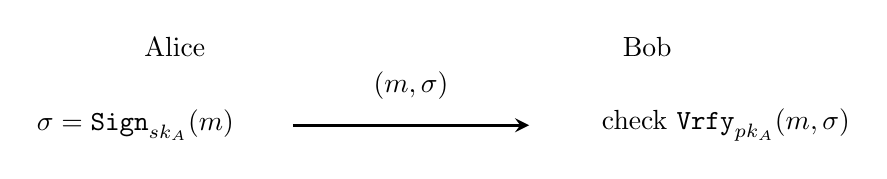
\begin{tikzpicture}[>=stealth]
			\node at (0, 1) {Alice};	
			\node at (3, .5) {$(m, \sigma)$};
			\draw[->,very thick] (1.5, 0) -- (4.5, 0);
			\node at (6, 1) {Bob};
			\node at (-.5, 0) {$\sigma = \texttt{Sign}_{sk_{A}}(m)$};
			\node at (7, 0) {$\text{check} ~ \texttt{Vrfy}_{pk_{A}}(m, \sigma)$};
		\end{tikzpicture}
	\end{center}

	\paragraph{Properties:}

	\begin{itemize}
		\item The signature is \emph{authentic} - Bob knows that Alice signed the
			message.
		\item The signature is \emph{unforgeable} - only Alice knows her private
			key.
		\item The signature is \emph{not reusable} for any other message -
			because it's a function of the message.
		\item Any \emph{alteration} of the message would invalid the signature -
			it won't be possible to verify the signature with Alice's public key anymore.
		\item The signature cannot be \emph{repudiated} - Alice cannot claim not
			having signed the message because she was the only one knowing her
			private key.
	\end{itemize}

	\subsection{Digital signature and timestamp}

	Digital signatures should also include timestamps (attach a timestamp to the
	message and sign the whole document). 

	Let's consider the following \emph{example}, taken from the Bruce Schneier's book
	“Applied Cryptography”:
	\begin{quotation}
		Alice sends Bob a signed digital check for \$100. Bob takes the check to
		the bank, which verifies the signature and moves the money from one
		account to another.
		The following week, Bob takes the same check to the bank, which again
		verifies the signature and moves the money from one account to another.
		And so on.

		But if date and time of signature are attached to the message, then the bank
		could store this timestamp into a database, and when Bob takes the check for
		the second time, the bank checks the timestamp against its database.
	\end{quotation}

	\subsection{RSA digital signature}

	\subsubsection{Naive RSA-signature}

	Alice's public key $\texttt{pk}_{A} = (n, e)$ and secret key is
	$\texttt{sk}_{A} = d$.

	\begin{center}
		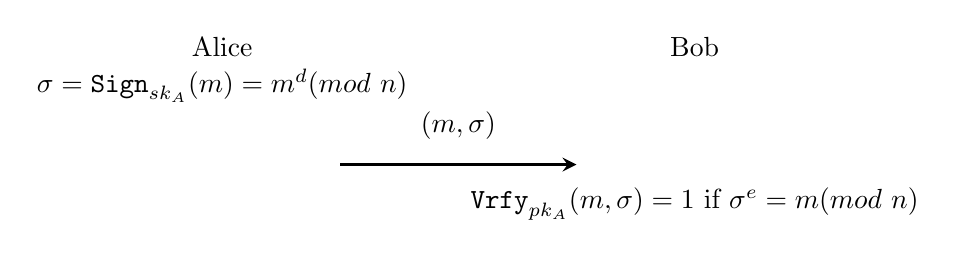
\begin{tikzpicture}[>=stealth]
			\node at (0, 1) {Alice};	
			\node at (3, 0) {$(m, \sigma)$};
			\draw[->,very thick] (1.5, -.5) -- (4.5, -.5);
			\node at (6, 1) {Bob};
			\node at (0, .5) {$\sigma = \texttt{Sign}_{sk_{A}}(m) = m^{d} (mod
			~ n)$};
			\node at (6, -1) {$\texttt{Vrfy}_{pk_{A}}(m, \sigma) = 1 ~ \text{if}
			~
			\sigma^{e} = m (mod ~ n)$};
		\end{tikzpicture}
	\end{center}

	\paragraph{Exercise 10.2.2} 

	Show that the above signature scheme is not secure.
	\emph{Hint}: choose any 
	$\sigma \in \mathbb{Z}_{n}$ and consider $m = \sigma^{e} (mod ~ n)$


	\vspace{10pt}

	First, let's remember what does it mean for a digital signature scheme
	to be \hyperlink{security}{secure}: 
	an adversary should not be able to produce a new message $m$ and a valid
	signature $\sigma$ for it. 

	Now, let's pick $\sigma \in \mathbb{Z}^{*}_{n}$. We define $m := \sigma^{e}
	(mod ~ n)$.
	Then it is true that:
	$$
		m = \sigma^{e} (mod ~ n) \quad \Longrightarrow \quad \sigma^{e} = m (mod ~ n)
	$$
	
	But this means that, by definition of our scheme,
	$\texttt{Vrfy}_{\texttt{pk}_{A}} (m, \sigma) = 1$, and therefore $\sigma$ is
	a valid signature for $m$.

	Now, some might argue that this isn't a realistic attack because the adversary 
	has not control over $m$. Actually this is irrelevant to our purposes: plain
	RSA signature doesn't respect digital signature security requisites.

	\subsection{EMSA-PSS - RSA digital signature}


	\emph{Encoding method for signature with appendix probabilistic signature
	scheme.} 
	(see also \url{https://tools.ietf.org/rfc/rfc3447.txt}).
	
	The following method is parametrized by the choice of:
	\begin{itemize}
		\item Hash function 
		\item Mask generation function
		\item Salt length
	\end{itemize}

	\begin{center}
		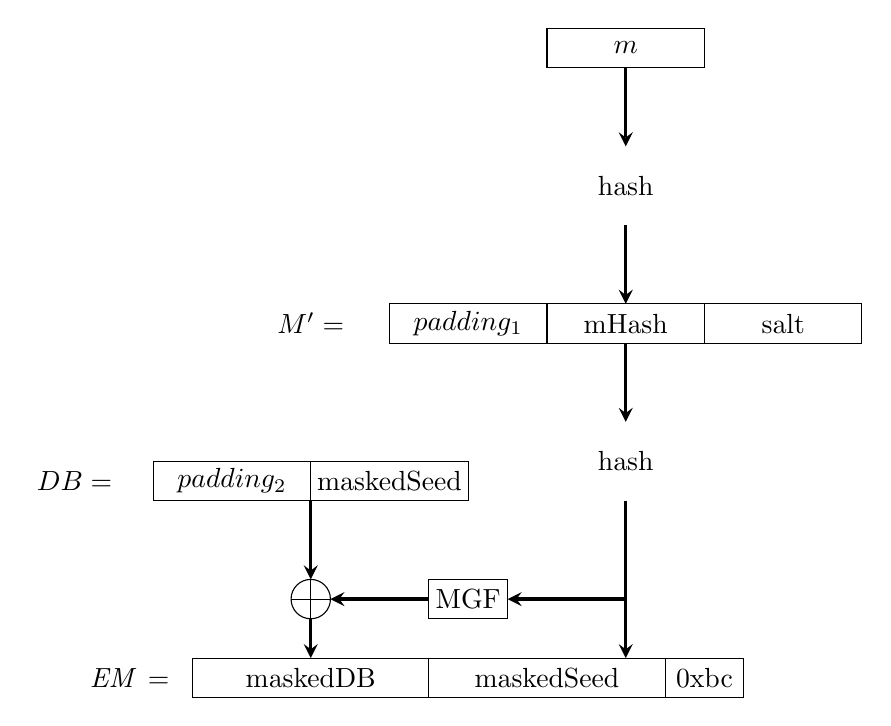
\begin{tikzpicture}[>=stealth]
			\draw (3, 6) rectangle +(2, .5);
			\node at (4, 6.25) {$m$};
			\draw[->,very thick] (4, 6) -- +(0, -1);
			\node at (4, 4.5) {hash};
			\draw[->,very thick] (4, 4) -- +(0, -1);
			\node at (0, 2.75) {$M' =$};
			\draw (1, 2.5) rectangle +(2, .5) node[pos=.5] {$padding_{1}$};
			\draw (3, 2.5) rectangle +(2, .5) node[pos=.5] {mHash};
			\draw (5, 2.5) rectangle +(2, .5) node[pos=.5] {salt};
			\draw[->,very thick] (4, 2.5) -- +(0, -1);
			\node at (4, 1) {hash};
			\draw[->,very thick] (4, .5) -- +(0, -2);
			\node at (-3, .75) {$DB=$};
			\draw (-2, .5) rectangle +(2, .5) node[pos=.5] {$padding_{2}$};
			\draw (0, .5) rectangle +(2, .5) node[pos=.5] {maskedSeed};
			\draw[->,very thick] (0, .5) -- +(0, -1);
			\draw[->,very thick] (4, -.75) -- +(-1.5, 0);
			\draw (1.5, -1) rectangle +(1, .5) node[pos=.5] {MGF};
			\draw[->,very thick] (1.5, -.75) -- +(-1.25, 0);
			\draw (0, -.75) circle (.25);
			\draw (-.25, -.75) -- +(.5, 0);
			\draw (0, -.5) -- +(0, -.5);
			\draw[->,very thick] (0, -1) -- +(0, -.5);
			\draw (-1.5, -2) rectangle +(3, .5) node[pos=.5] {maskedDB};
			\draw (1.5, -2) rectangle +(3, .5) node[pos=.5] {maskedSeed};
			\draw (4.5, -2) rectangle +(1, .5) node[pos=.5] {0xbc};
			\node at (-2.3, -1.75) {\emph{EM }=};
		\end{tikzpicture}
	\end{center}

	Let's first define fundamental component:
	\begin{itemize}
		\item \texttt{emLen} = length of the encoded message (EM) 
			(at least $8\cdot \texttt{hLen} + 8\cdot \texttt{sLen} + 9$).
		\item \texttt{hLen} = length of $\texttt{mHash} = \texttt{hash}(m)$.
		\item \texttt{sLen} = length of \texttt{salt}.
		\item $padding_{1}$ = \texttt{0x0000000000000000} 
		\item $padding_{2}$ = \texttt{PS || 0x01} where \texttt{PS} is an octet
			string consisting of \texttt{emLen - sLen - hLen - 2} zero octets
			(bytes).
	\end{itemize}


	\paragraph{Encoding:}

	\begin{enumerate}
		\item If the length of $m$ is greater than the input limitation for the 
			hash function ($2^{61} - 1$ octets for SHA-1), output "message
			too long" and stop.
		\item Let \texttt{mHash = Hash(M)}, an octet string of length \texttt{hLen}.
		\item If \texttt{emLen} \texttt{< hLen + sLen + 2}, output "encoding error" 
			and stop.
		\item Generate a random octet string salt of length \texttt{sLen}; if
			\texttt{sLen = 0},
			then \texttt{salt} is the empty string.
		\item Let
			\texttt{M'} = \texttt{0x 00 00 00 00 00 00 00 00} || \texttt{mHash} || 
			\texttt{salt}.
			\texttt{M'} is an octet string of length \texttt{8 + hLen + sLen} with
			eight initial zero octets.
		\item Let \texttt{H = Hash(M')}, an octet string of length \texttt{hLen}.
		\item Generate an octet string \texttt{PS} consisting of\texttt{emLen - sLen - hLen - 2} 
			zero octets.  The length of \texttt{PS} may be 0.
		\item Let \texttt{DB = PS || 0x01 || salt}; \texttt{DB} is an octet string of length
			\texttt{emLen - hLen - 1}.
		\item Let \texttt{dbMask = MGF(H, emLen - hLen - 1)}.
		\item Let \texttt{maskedDB} = \texttt{DB} $\oplus$ \texttt{dbMask}.
		\item Set the leftmost \texttt{8emLen - emBits} bits of the leftmost octet in
			\texttt{maskedDB} to zero.
		\item Let \texttt{EM = maskedDB || H || 0xbc}.
		\item Output \texttt{EM}.
	\end{enumerate}

	 Verification operation follows reverse steps to recover \texttt{salt}, then forward 
	 steps to recompute and compare \texttt{H}. 

	\paragraph{Exercise 10.2.4}
	Find $padding_{2}$ in the standard.


	\subsection{Digital signature algorithm}

	In 1991, The National Institute of Standards and Technology (NIST) proposed
	the Digital Signature Algorithm (DSA) for use in their Digital Signature
	Standard (DSS).


	We consider a bit length of 1024, though longer bit lenghs are possible in
	the standard.

	\subsubsection{Key generation}

	\begin{enumerate}
		\item Generate a prime number $p$ with $2^{1023} < p < 2^{1024}$.
		\item Find a prime divisor $q$ of $p-1$ with $2^{159} < q < 2^{160}$.
		\item Find an element $\alpha$ with $ord(\alpha) = q$, i.e. $\alpha$
			generates the subgroup with $q$ elements\footnote{Remember that a
			group is a set of elements with a binary operation defined on it,
			and the properties of closure (i.e. the operation is closed), 
			associativity, neutral element, inverse element, while the \emph{order} 
			of an element $\alpha$ of the group is the smallest positive integer $k$
			such that $\alpha^{k}$ = 1, where $1$ is the neutral element of the
			group.}
		\item Choose a random integer $d$ with $0 < d < q$.
		\item Compute $\beta \equiv \alpha^{d} ( mod ~ p )$
		\item The keys are $k_{pub} = (p, q, \alpha , \beta)$ and $k_{pri}= d$.
	\end{enumerate}

	\paragraph{Generating large prime numbers}

	How do we generate a prime number $p$ such that $2^{1023} < p < 2^{1024}$?
	We can observe that $2^{1023}$ is just $1$ followed by 1023 zeros, i.e.
	$1000...0$. To pick a random number between $2^{1023} and 2^{1024}$ we can
	just set to 1 some random zero-bits: the resulting number will be in the
	given range.

	\subsubsection{Signature}

	\begin{enumerate}
		\item Choose an integer as random \emph{ephemeral}\footnote{An ephemeral
			key or \emph{session} key is a key valid only for a limited period
			of time, usually the time of a connection between two hosts.} key 
			$k_{E}$ with 0 < $k_{E}$ < $q$.
		\item Compute $r \equiv (\alpha ^{k_{E}} (mod ~ p)) (mod ~ q)$
		\item Compute $s \equiv (SHA(x) + d \cdot r) k^{-1}_{E} (mod ~ q)$
	\end{enumerate}

	Where $x$ is the message to be signed.

	\subsubsection{Verification}

	\begin{enumerate}
		\item Compute auxiliary value $w \equiv s^{-1} (mod ~ q)$
		\item Compute auxiliary value $u_{1} \equiv w \cdot SHA(x) (mod ~ q)$
		\item Compute auxiliary valid $u_{2} \equiv w \cdot r (mod ~ q)$
		\item Compute $v \equiv (\alpha^{u_{1}} \cdot \beta^{u_{2}} (mod ~ p) )(mod ~ q)$
		\item The verification $ver_{k_{pub}}(x, (r, s))$ follows from:
			$$
			v \begin{cases}
				\equiv r (mod ~ q) & \Rightarrow \text{valid signature} \\
				\not\equiv r (mod ~ q) & \Rightarrow \text{invalid signature} \\
			\end{cases}
			$$
	\end{enumerate}

	I.e. the verifier accepts a signature $(r, s)$ only if $v \equiv r (mod  ~
	q)$ is verified.

	\paragraph{Exercise 10.3.6}

	Set $p = 59, q = 29, \alpha = 3, d = 7, \beta = \alpha^{d} (mod ~ 59)$.
	Assuming that $SHA(x) = 26$ compute the DSA signature $(r, s)$.

	\vspace{20pt}

	\begin{enumerate}
		\item We choose $k_{E} = 7$
		\item We compute $r$ as:
			$$
				(\alpha^{k_{E}}(mod ~ p)) (mod ~ q) = 
				(3^{7} (mod ~ 59)) (mod ~ 29) = 4
			$$
		\item We compute $s$ as:
			$$
				(SHA(x) + d\cdot r) \cdot k_{E}^{-1} (mod ~ q) = 
				(26 + 7 \cdot 4) \cdot 7^{-1} (mod ~ 29) = 
				7
			$$
	\end{enumerate}

	So the digital signature is $(r, s) = (4, 7)$.

	\paragraph{Exercise 10.3.7}

	If an adversary is able to predict $k_{E}$ DSA is broken. Read the following
	article: \url{https://www.bbc.com/news/technology-12116051}.

	\paragraph{Exercise 10.3.8}

	Consider a variant of DSA in which just messages in $\mathbb{Z}_{q}$ are signed 
	and the Hash function is omitted, i.e. to get the signature $(r,s)$ of $m \in
	\mathbb{Z}_{q}$ we compute $r=\alpha^{k_{E}}$ (as  usual), but
	$s= (m+d\cdot r)\cdot k^{-1}_{E}(mod ~ q)$.  Is this secure?

	\vspace{20pt}

	A possible attack can be done by setting $k_{E} = d$. The attacker doesn't
	know the secret key $d$, but now it has to output $s = (m + d \cdot
	r) d^{-1} (mod ~ q)$. He or she can just choose $m = 0$, so that:
	$$
		s = (m + d \cdot r) d^{-1} (mod ~ q) = (d \cdot r) \cdot d^{-1} (mod ~ q) 
		= r (mod ~ q)
	$$

	Now $s$ can be computed, because it only depends on known parameters, 
	and $(r, s)$ with $r = s$ is a valid signature for $m$.

	\subsubsection{Prime generation for DSA}

	The following is a slightly different generator taken from “Understanding
	Cryptography” by Christof Paar. The goal here is to find two primes $(p, q)$
	where $2^{1023} < p < 2^{1024}$ and $2^{159} < q < 2^{160}$ and $p-1$ is a
	multiple of $q$:

	\renewcommand{\labelenumii}{\arabic{enumi}.\arabic{enumii}.}

	\vspace{10pt}

	\textbf{Initialization:} Set i = 1.

	\begin{enumerate}
		\item Find prime $q$ with $2^{159} < q < 2^{160}$ using the Miller-Rabin
			algorithm\footnote{Miller-Rabin algorithm is a primality test for
			numbers.}.
		\item For i = 1 to 4096:
			\begin{enumerate}
				\item Generate a random integer $M$: $2^{1023} < M < 2^{1024}$.
				\item $M_{r} \equiv M (mod ~ 2q)$
				\item $p-1 \equiv M - M_{r}$ (note that $p-1$ is a multiple of
					$2q$)
				\item if $p$ is prime return$(p, q)$
				\item i = i+1
			\end{enumerate}
		\item Go back to step 1.
	\end{enumerate}



\end{document}
